This section describes the implementation of SESH into SAMMY as required for fitting resonance parameters to self-shielded URR measurements.

This chapter details the implementation of a new, fully integrated workflow within the SAMMY resonance parameter fitting code. The primary motivation for this work was to overhaul the previous method for analyzing self-shielded measurements in the URR. 

Previously, evaluating URR data was a tedious, manual cycle, requiring the user to go back and forth between SAMMY and SESH. The process, shown in \autoref{fig:original-self-shielding-workflow}, required the user to convert a transmission measurement $\langle T \rangle$ to a non-physical ``uncorrected'' cross section:
\begin{equation}
    \overline{\sigma} = -\frac{1}{n} \ln{ \langle T \rangle}
\end{equation}
This derived value, which as previously states is not the true cross section, but the self-shielded cross section, is dependent on experimental conditions (sample thickness, sample temperature, sample composition, etc.), and needed to be corrected in order to be fit with SAMMY.
\begin{figure}
    \centering
    \includegraphics[width=0.75\linewidth]{Implementation/Figures/SelfShieldingWorkflow.png}
    \caption{Original Self-Shielding Correction Workflow for Fitting in URR}
    \label{fig:original-self-shielding-workflow}
\end{figure}
This was converted into the \textit{true} average cross section by use of the correction factor calculated from SESH, which was then fit with SAMMY.

Once new parameters were obtained, they were used to calculate a new correction factor. This was then used to obtain a new `corrected' cross section, and a new fit was performed, producing new resonance parameters. This process was repeated until the resonance parameters converged onto a final value.

The implementation described in the following sections integrates the self-shielding correction capabilities of SESH directly into SAMMY’s fitting engine. This creates a new, streamlined workflow where the evaluator provides the actual measurement data—such as average transmission or capture yield—directly to the code. SAMMY now internally calculates the necessary self-shielding correction factors during each iteration, directly comparing the theoretical values to the experimental observable. The new and improved workflow is shown in \autoref{fig:current-workflow}.
\begin{figure}[h]
    \centering
    \includegraphics[width=1\linewidth]{Implementation/Figures/improved-workflow.png}
    \caption{Current SAMMY workflow for processing self-shielded URR data}
    \label{fig:current-workflow}
\end{figure}

While the code SESH was used to provide a blueprint for performing self-shielding corrections, its implementation into SAMMY required a near-total rewrite of the original code. This overhaul was required in order to modernize SESH's interface such that it integrated cleanly into SAMMY, resolve bugs that had been propagated through SESH's development history, and improve the physics models such that:
\begin{enumerate}
    \item Approximations which significantly impacted results were removed
    \item SESH and SAMMY utilize the same underlying physics models, ensuring consistency throughout the code.
\end{enumerate}

The following sections will discuss software refactoring (bug fixes, improved physics models) required to perform the self-shielding corrections in order to accomplish these goals. The specific theoretical measurement validation will be discussed in their respective chapters, as will the fitting procedure.

\section{URR Representation in SAMMY}
\label{sec:urr-in-sammy}

The average cross section in the URR is typically defined according to Hauser-Feshbach theory, which provides a framework for describing nuclear reactions proceeding through a compound nucleus when many channels are open and individual resonance effects are smeared out. The energy-averaged total cross section for an incoming channel $c$ can be expressed as:

\begin{equation}
    \label{eq:hauser-feshbach-cross-section}
    \langle \sigma_c \rangle =
    2 \pi \lambdabar_c^2 g_c \left\{
    1 - \frac{
            \cos{ ( 2 \phi_c)} \left[
                1 - \pi^2P_c^2 s_c^2 -  \left( P_c R_c^\infty \right)^2
            \right]
            + \sin{(2 \phi_c)} 2 P_c R_c^\infty
        }{
            \left( 1 + \pi P_c s_c \right)^2 + \left( P_c R_c^\infty \right)^2
    }
    \right\} \quad \text{}
\end{equation}
In this formulation, $\lambdabar$ is the reduced de Broglie wavelength for the neutron, $g_c$ is the statistical spin factor defined as $g_c = \frac{2J + 1}{2(2I + 1)}$ where $I$ is the spin of the target nucleus , and $\phi_c$ is the hard-sphere scattering phase shift for a particular channel. The form of $\phi_c$ depends on the orbital momentum $\ell$ and is a function of $\rho = \frac{a_c}{\lambdabar}$, where $a_c$ is the scattering radius of the target nucleus.

The parameters of significance to transmission self-shielding in the URR, which distinguish this average cross section from a simple energy average of RRR cross sections, are the distant level parameter $R^\infty_c$ and the strength function $\Tilde{S}_c$. Here, $P_c$ is the neutron penetrability, and $s_c$ is the pole strength, defined as $s_c = \Tilde{S}_c\lambdabar a_c \sqrt{E}/2$. The strength function $\Tilde{S}_c$ characterizes the average reduced width of resonances for a given orbital $\ell$.


\section{Converting from SAMMY Parameters to SESH Parameters}
    As shown in \autoref{sec:mc-sampling-from-average-parameters}, accurately modeling resonance self-shielding requires stochastically sampling resonances to account for cross-section variance. While \autoref{eq:hauser-feshbach-cross-section} provides a convenient analytical form for the average cross-section, it doesn't account for that variance. 
    
    This presents a significant challenge. The URR parameters as input to SAMMY, such as the strength function $S_\ell$, distant-level parameter $R_\ell^\infty$, and s-wave level spacing $D_0$, are all defined on an orbital momentum $\ell$ basis. These $\ell$-dependent terms are very convenient to use for the average cross-section, but cannot generate resonances directly. Actual nuclear resonances are tied to particular quantum states, or channels, each defined by a unique $J$ (spin), $\ell$ (orbital momentum), and $\pi$ (parity) combination.

    There's three major conversions that need to be done:
    \begin{enumerate}
        \item Convert $D_0$ to $D_J$
        \item Convert $S_\ell, D_J$ to $\langle \Gamma_{n,J}^\ell \rangle$
        \item Convert $R_\ell^\infty$ to $R'$ (for use in calculating the hard-sphere phase shift)
    \end{enumerate}
    The following sections describe this conversion process in order to perform channel-by-channel resonance simulation.


    \subsection{Calculating Available Channels}
        \label{ssec:channels}
    
        For an isotope with a ground-state spin $I$ interacting with a neutron (which has an intrinsic spin of $s_n = 1/2$), there are two possible channel spins: $s_{-} = I - 1/2$ and $s_{+} = I + 1/2$. This leads to two separate cases for the total angular momentum $J$: one for $s_{-}$ and one for $s_{+}$:
        \begin{align}
            \mathbf{J}_{-} &= \left\{ \left|s_{-} - \ell\right|, \left|s_{-} - \ell\right| + 1, \cdots, s_{-} + \ell \right\}\\
            \mathbf{J}_{+} &= \left\{ \left|s_{+} - \ell\right|, \left|s_{+} - \ell\right| + 1, \cdots, s_{+} + \ell \right\}
        \end{align}
        One common assumption is that spin-group parameters are assumed to be independent of parity\cite{endf-manual}, i.e., $(J, \ell, -1) = (J, \ell +1)$. As a consequence, only $J$ and $\ell$ need to be considered when calculating resonances. Instead, the important factor to consider is the degrees of freedom, or the multiplicity, $\mu$. If the same $J,\ell$ combination can be calculated from $s_{+}$ and $s_{-}$ channel spins, then $\mu_i = 2$. Otherwise, $\mu_i=1$. This overlap is illustrated in \autoref{eq:multiplicities}:
        \begin{equation}
            \label{eq:multiplicities}
            \begin{array}{rrrrrrrr}
            \mathbf{J}_{-}: & \{ & \left|s_{-} - \ell\right|, & \left|s_{-} - \ell\right| + 1, & \dots, & s_{-} + \ell ~ & & \} \\
            \mathbf{J}_{+}: & \{ & & \left|s_{+} - \ell\right|, & \dots, & s_{+} + \ell-1, & s_{+} + \ell & \} \\[1em] \hline \\[-0.5em]
            \mathbf{J}_{tot}: & \{ & \left|s_{-} - \ell\right|, & \left|s_{+} - \ell\right|, & \dots, & s_{-} + \ell, & s_{+} + \ell & \} \\
            \mathbf{\mu}_J: & \{ & 1, & 2, & \dots, & 2, & 1 & \} \\
            \end{array}
        \end{equation}
        The purpose for this `once-over' approach is that it significantly reduces the number of channels being sampled. Instead of generating two separate resonances, only a single resonance is sampled. The only modification required is to sample neutron widths from the Porter-Thomas distribution using the given multiplicity as its degrees of freedom. By utilizing this assumption, the number of required sampling events can be nearly halved.
    
        The total vector of unique available channels, $\mathbf{C}$ is then created by compiling the $\mathbf{J}_{tot}$ and $\mathbf{\mu}_J$ vectors for each given $\ell$ value. The elements of $C$ are given as:
        \begin{equation}
        \label{eq:channel=list}
            c_i = (J_i, \ell_i, \mu_i)
        \end{equation}
        which describes the complete set of quantum states available for a given nucleus.

    \subsection{Improving Level Density J Dependency}
        \label{ssec:level-density}
        With the set of available channels established, the next step is determining the average level spacing, $D$ for each channel. This calculation is simplified by two key properties. The first is that average level spacing is observed to be independent of $\ell$\cite{level-spacing-statistics}. The second is the previous assumption that was made, in that average channel parameters are independent of parity, $\pi$. This means that the only parameter in which average level spacing is dependent is $J$, or
        \begin{equation}
            D_{\ell,J,\pi} = D_J
        \end{equation}
        and therefore only $J$ dependence needs to be accounted for when calculating channel-by-channel level-spacings.
        
        A significant update was implemented in the methodology for determining the $J$-dependent level spacing, $D_J$. SESH calculated this value  using a simple relation involving the statistical spin factor, $g_J$, as
        \begin{equation}
            \label{eq:simple-j-dependency}
            D_J = \frac{D_0}{g_J}
        \end{equation}
        and where $D_0$ is the user-input S-wave level spacing. The primary motivation for this change was to eliminate previous approximations which SESH utilized for this formula to enable a more physically realistic model that accounts for energy dependency of level spacings across different $J$ values.
        
        The updated methodology uses the same input S-wave level spacing, but instead uses Betha formula to describe the conversion from $D_0$ to $D_J$
        \begin{equation}
            \label{eq:bethe-formula}
            \frac{1}{D_J} = \frac{1}{D_0}
            \left\{ \exp{ \left[ \frac{-J^2}{2\sigma(E)^2}\right]} - \exp{ \left[ \frac{-(J+1)^2}{2\sigma(E)^2}\right]} \right\} 
        \end{equation}
        where $\sigma$ is the spin cutoff factor, which is described by
        \begin{equation}
            \sigma^2 = (0.14592)(A+1)^{2/3}\sqrt{a(E + BE - PE)}
        \end{equation}
        This allows for a significantly improved model that permits $D_J/D_0$ to evolve as a function of energy more realistically compared to the simple SESH formula.
        
        The energy dependence of $D_0$ is also accounted for with the Gilbert-Cameron level density model\cite{gc-leveldensity}. This had already matched the SAMMY implementation, and therefore was left unchanged.

        The validation of this model was done by comparing the new calculated level densities with the new \textsuperscript{181}Ta evaluation from ENDF-8.1\cite{endf-8.1}.

        \begin{figure}[H]
            \centering
            \begin{adjustbox}{width=1.2\textwidth, center}
            \includegraphics{Implementation/Figures/validating-level-spacing.png} 
            \end{adjustbox}
            \caption{Validating the improved level spacing model in SESH with \textsuperscript{181}Ta spin groups from ENDF-8.1 Evaluation}
            \label{fig:level=spacing=validation}
        \end{figure}

        As shown in \autoref{fig:level=spacing=validation}, the results from the improved SESH level density formula now correctly matches the evaluation. While the simpler model for \autoref{eq:simple-j-dependency} approximates the level spacing for the S-wave associated channels, the two formulas become more discrepant at higher $\ell$ values. Implementing \autoref{eq:bethe-formula} resolves the approximations that were inherent in SESH.

        It should also be noted that \textsuperscript{181}Ta has a relatively well-behaved URR. The disagreement between the two formulas would be much larger for nuclei with less-than-ideal URRs (e.g., \textsuperscript{90}Zr).

    \subsection{Converting Strength Functions to Neutron Widths}
        With the complete set of available channels and the $J$ and $E$ dependent level spacings calculated in the previous sections, the per-channel neutron width can be calculated. The average neutron width, $\langle \Gamma_{n,J}^{\ell} \rangle$ can be calculated. This quantity is calculated for each unique $(\ell,J)$ by:
        \begin{equation}
            \label{eq:avg-neut-width}
            \langle \Gamma_{n,J}^{\ell} \rangle = \mu_{\ell,J} D_J S_\ell \nu_{\ell}(E) \sqrt{E}
        \end{equation}
        in which $S_\ell$ is the strength function, and $\nu_{\ell}$ is the penetrability, which has an $\ell$ and $\rho$ dependent form given in \autoref{eq:penetration-factor}.
        \begin{equation}
        \label{eq:penetration-factor}
            \nu_\ell = \begin{cases}
                \quad\quad\:\:\:\displaystyle\rho & \ell=0,\\[12pt]
                \quad\:\:\displaystyle\frac{\rho^3}{1 + \rho^2} & \ell=1,\\[12pt]
                \displaystyle\frac{\rho^5}{9 + 3\rho^2 + \rho^4} & \ell=2\\
                %&\displaystyle\frac{\rho^7}{225 + 45\rho^2 + 6\rho^4 + \rho^6} & \ell=3
            \end{cases}
        \end{equation}

        The parameter $\rho$ is the is the center-of-momentum of the reaction, defined as
        \begin{equation}
            \rho = k a_c
            \label{eq:center-of-momentum}
        \end{equation}
        in which $a_c$ is the scattering radius of the target nucleus, and $k$ is the neutron wave number.

        Putting all of these pieces together, the average neutron with is calculated from input parameters. This parameter is what's fed into \autoref{eq:porter-thomas} to generate samples of the neutron width for simulating self-shielding.
        
    \subsection{Converting Inelastic Strength to Inelastic Widths from Channels}
        \label{ssec:inelastic-strength}
        Originally in SESH, the inelastic contribution was determined using an identical form to \autoref{eq:avg-neut-width}, and the average value was used without modification.

        This approach is a poor physical approximation as it fails to account for the discrete nature of nuclear excited states. The ENDF-6 manual\cite{endf-manual} provides guidance in calculating the inelastic width. This is implemented in the code as:
        \begin{equation}
            \label{eq:inelastic-width}
            \langle \Gamma_{n',J}^\ell \rangle = \sum_{i,\ell'} = \mu_{J,\ell'} D_J S_{\ell'} \nu_{\ell'}(E - E_i)
        \end{equation}
        Here, the sum is over all excited states $i$ and all possible outgoing orbital momenta $\ell'$. This more realistically accounts for the inelastic neutron width than the original SESH formula, and is in agreement with SAMMY's calculated inelastic widths.

    \subsection{Calculating Potential Scattering}
        \label{ssec:pot-scat}

        The final component required for the cross-section simulation is the potential scattering. As shown in \label{eq:slbw}, the first part of that equation exists outside the resonance sum. This is the potential scattering term\cite{t2}, and can be written as
        \begin{equation}
            \label{eq:potential-scattering}
            \sigma_p = \frac{ 4 \pi}{k^2} \sum_\ell (2\ell +1) \sin^2{\phi_\ell}
        \end{equation}
        The key to this equation is $\phi_\ell$, the hard-sphere phase shift, which is calculated as a function of $\ell$ and $\hat{\rho}$, as described in
\autoref{eq:phase-shift}.

    \begin{equation}
        \label{eq:phase-shift}
        \phi_\ell = \begin{cases}
            \hat{\rho} & \ell=0,\\[12pt]
            \hat{\rho} - \arctan{\hat{\rho}} & \ell=1,\\[12pt]
            \displaystyle\hat{\rho} - \arctan{\frac{3\hat{\rho}}{3 - \hat{\rho}} } & \ell=2\\[12pt]
            %\displaystyle{\hat{\rho} - \arctan{\frac{15\hat{\rho} - \hat{\rho}^3}{15 - 6\hat{\rho}^2} } }  & \text{if}\quad \ell=3\\[14pt]
        \end{cases}
    \end{equation}

        The term $\hat{\rho}$ is solved similarly to $\rho$ from \autoref{eq:center-of-momentum}. However, rather than using the channel radius $a_c$, it uses the effective scattering radius, $R'$:
        \begin{equation}
            \hat{\rho} = kR'
        \end{equation}
        The effective scattering radius is where the given $R^\infty_\ell$ term gets utilized.

        In the low-energy limit, the effective scattering radius for s-waves, \textit{R'}, can be calculated from the channel radius, $a_c$, and the distant level parameter, $R_0^\infty$, using the well-known approximation:
        \begin{equation}
            R' = a_c (1 - R_0^\infty) \label{eq:1}
        \end{equation}
        However, for analyses that extend to higher energies or include higher orbital momenta $(\ell > 0)$, this s-wave approximation is considered inadequate\cite{jeff18}. A more sophisticated model is required to accurately replicate the underlying cross-section behavior and its associated resonance structure.
        
        The generalized SPRT method\cite{sprt} provides an improved model that addresses the s-wave low-energy approximation. It offers an approximate relationship for the effective radius, $R_l'$, which accounts for the variation with higher-order partial waves:
        \begin{equation}
            R_l^{\prime} \approx a_c\left[1-(2 l+1) R_l^{\infty}\right]^{1 /(2 l+1)}
        \end{equation}
        This equation provides a more suitable description for cases where partial waves beyond \textit{l}=0 make a significant contribution.

\section{Validation of the Weighted Wigner Distribution}
As detailed in \autoref{sec:sampling-parameters}, generating a statistical resonance ladder involves sequentially  sampling level spacings, $s$, from the Wigner distribution given at \autoref{eq:wigner-distribution}. However, building whole ladders would be extremely inefficient for SESH's purposes. While NJOY and FRENDY need to sample across the entire URR, SESH is designed to correct at specific energies.

To circumvent this inefficiency, only the resonances directly around the energy of interest are sampled. The issue with doing this is that a neutron is proportionally more likely to fall into a wider level spacing than a narrow one, assuming a uniform energy distribution. To address this, Fr\"{o}hner developed a weighted sampling scheme to sample level spacings weighted by their size, which can be represented as:
\begin{equation}
    \label{eq:weighted-wigner}
    P_{weighted}(s) = \frac{s \cdot P(s)}{\displaystyle\int_0^\infty s' \cdot P(s') ds'}
\end{equation}

In order to validate Fr\"{o}hner's implementation of \autoref{eq:weighted-wigner}, a sequence of $10^7$ resonances was built,
\begin{equation}
    \left\{\lambda_0, \lambda_1, \lambda_2, \dots, \lambda_{N-1}, \lambda_{N} \right\}
\end{equation}
in which
\begin{equation}
    \lambda_{r+1} = \lambda_r + s_r
\end{equation}
where $s_r$ was sampled from \autoref{eq:wigner-distribution}. A random energy $E_{rand}$ was randomly sampled from a uniform distribution over the range $[\lambda_0,\lambda_N]$, and identified a resonance $i$ which fit the criteria:
\begin{equation}
    \lambda_i \leq E_{rand} < \lambda_{i+1}
\end{equation}
Therefore, the sampled $s_{selected}$ was determined by:
\begin{equation}
    s_{observed} = \lambda_{i+1} - \lambda_{i}
\end{equation}
This observed width was collected into a set and compared to the sampled values from Fr\"{o}hner's implementation of \autoref{eq:weighted-wigner}.
\begin{figure}[H]
    \centering
    \includegraphics[width=0.75\linewidth]{Implementation/Figures/weighted-wigner-validation.png}
    \caption{Validation of Frohner's implementation of the weighted Wigner level spacing algorithm}
    \label{fig:weighted-wigner}
\end{figure}

As shown in \autoref{fig:weighted-wigner} Fr\"{o}hner's implementation of the weighted Wigner distribution successfully replicates the distribution of observed widths when weighting according to energy, and can be used to accelerate the sampling routine without a loss of accuracy.

\section{Doppler Broadening}

When testing SESH theoretical values, there was an observed disagreement in cross-section variance at higher energies for capture cross sections.
    The primary cause of the disagreement was determined to be the result of an error in the Doppler broadening subroutine that was originally present in SESH. In order to perform the Doppler broadening, the complex error function, also known as the Faddeeva function, is utilized. The issue was in the original algorithm, in cases where $\beta$ was less than 0.01. Recall that
    \begin{equation}
        w(\alpha,\beta) = \frac{i}{\pi} \int_{-\infty}^{\infty} \frac{e^{-t^2}}{\alpha + i\beta - t}dt
    \end{equation}
    and
    \begin{equation}
        \beta = \frac{\theta}{2} = \frac{\Gamma_{tot}}{4\sqrt{\frac{ \kappa T E}{A}}}
        \label{eq:doppler-beta}
    \end{equation}

    In instances where $\beta \leq 0.01$, the algorithm would incorrectly return the 0 Kelvin value for the $\psi$ parameter, shown in \autoref{fig:beta-error}.
    \begin{figure}[h]
        \centering
        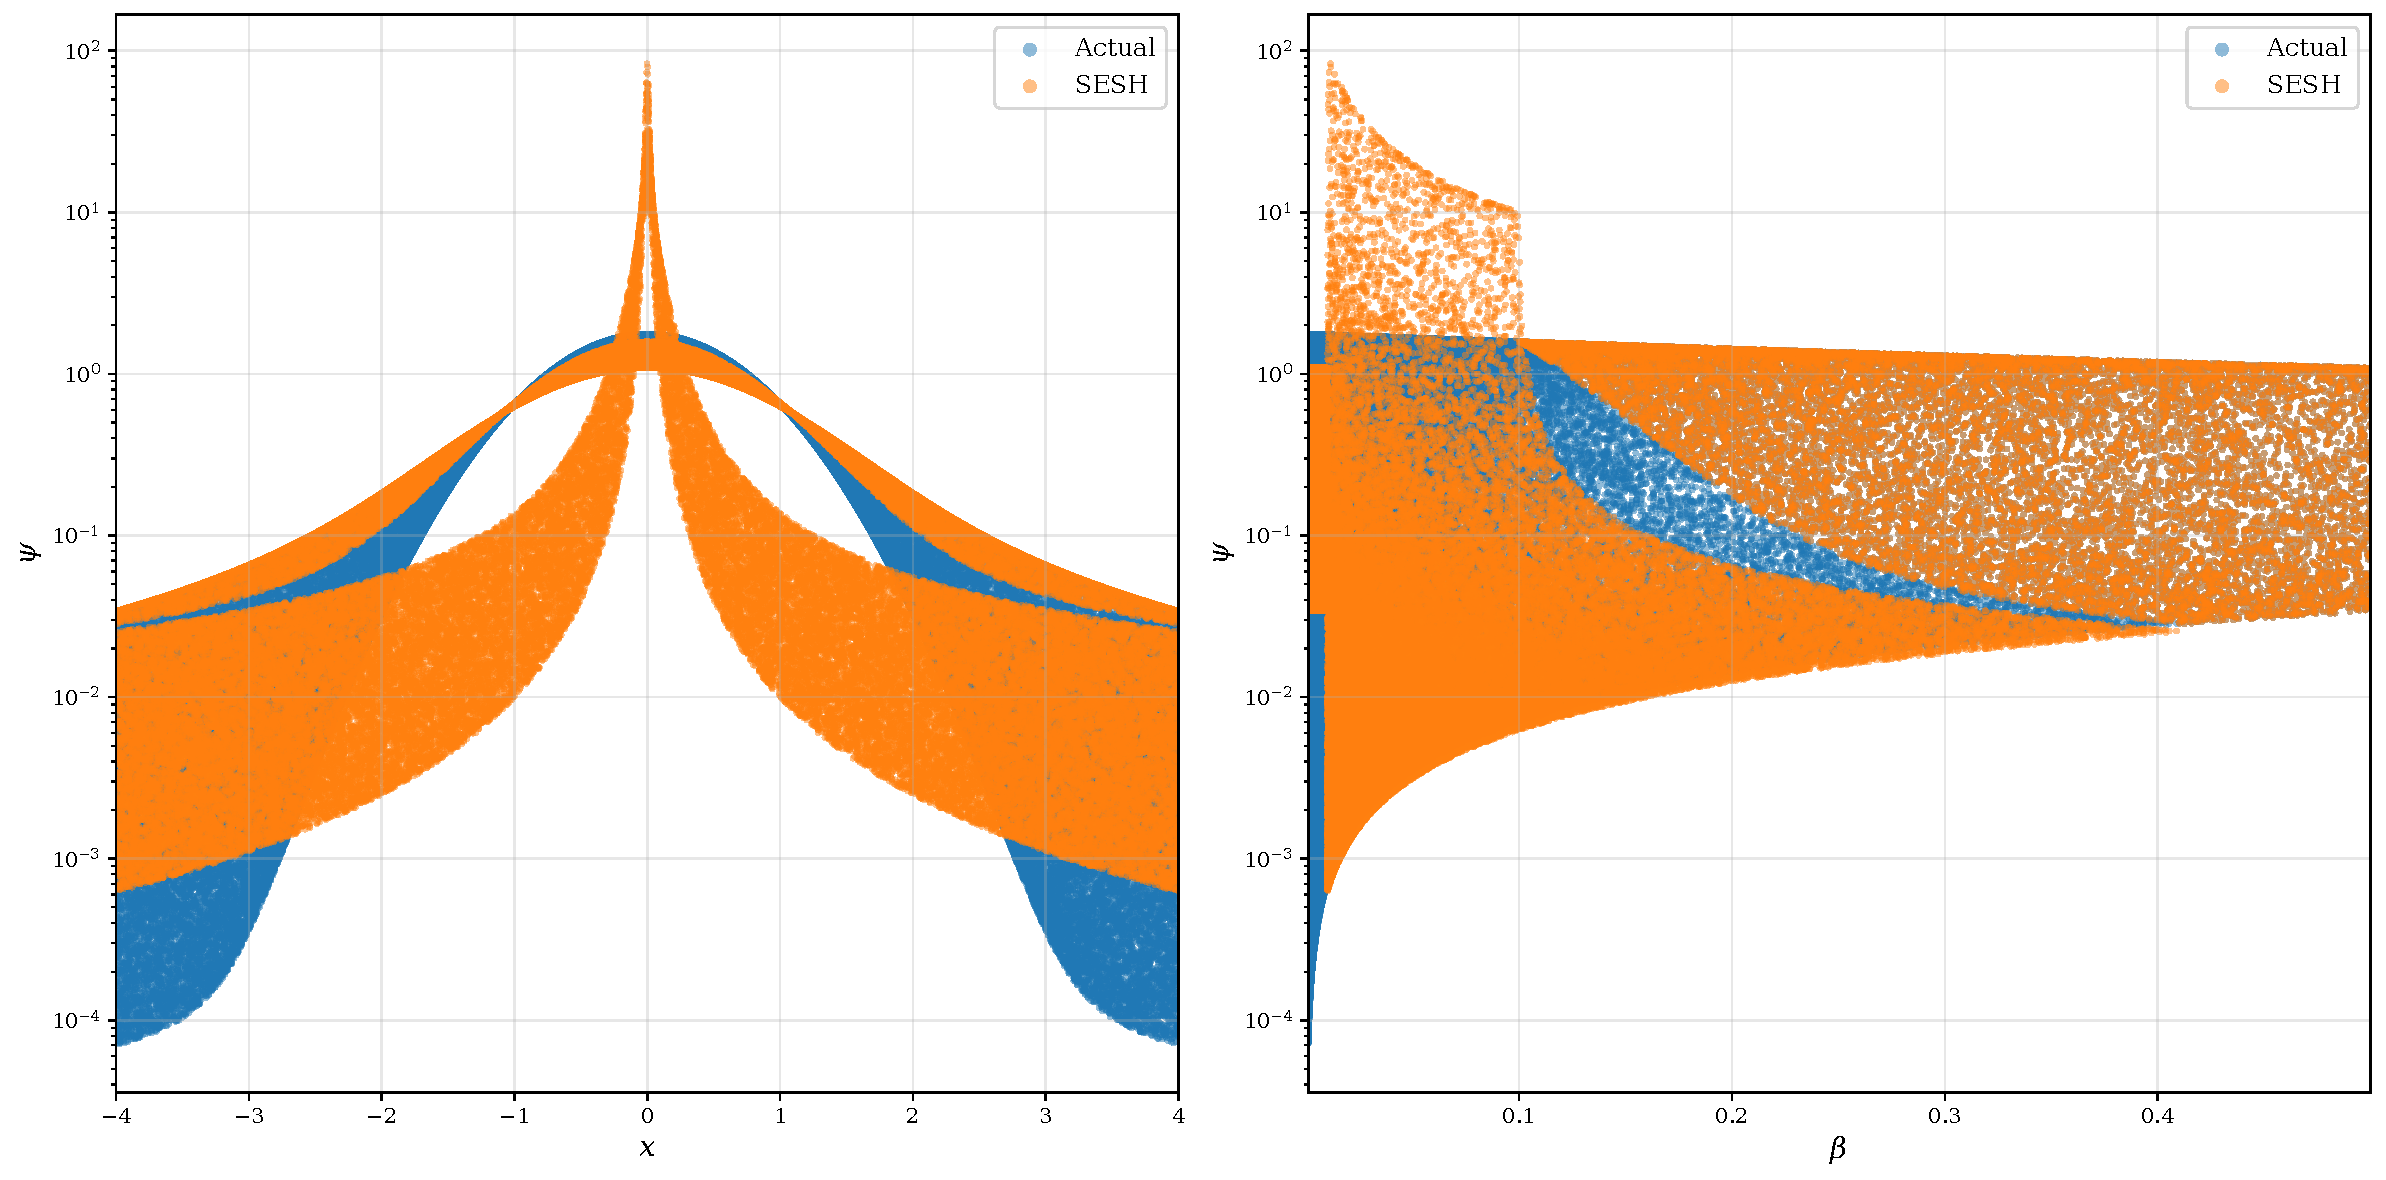
\includegraphics[width=0.75\linewidth]{Implementation/Figures/beta-error.png}
        \caption{Comparing results of SESH's Faddeeva function output with what the Faddeeva function actually calculates given the same inputs.}
        \label{fig:beta-error}
    \end{figure}
    
    One significant effect of this bug is due to the inverse relationship between $\beta$ and energy, shown in \autoref{eq:doppler-beta}. As the energy of the incident neutron increases, the probability of $\beta$ being sampled as less than 0.01 increases. Consequently, as energy increases, the probability of the 0 Kelvin cross section being returned also increased.

    The solution was to implement a newer computation of the Faddeeva function\cite{faddeeva}. This resolved the issues present in the original algorithm present in SESH, but also reduced error of the function at all values of $\beta$, shown in \autoref{fig:faddeeva-algorithm}.
    \begin{figure}[H]
        \centering
        \includegraphics[width=0.75\textwidth]{Implementation/Figures/DopplerBroadenedBeta.png}
        \caption{Faddeeva function error for old and new algorithms as a function of $\beta$.}
        \label{fig:faddeeva-algorithm}
    \end{figure}

\section{Cross-Section Validation}
    \label{sec:cross-section-validation}
    After the comprehensive refactoring of the SESH code, it was necessary to validate its performance in calculating cross-section distributions. The goal was to ensure that the updated SESH could accurately reproduce cross-section distributions from the same set of resonance parameters.

    In order to perform this validation, the cross-section distribution of \textsuperscript{90}Zr at 200 keV was generated by SESH and FRENDY\cite{frendy}. Rather than using the \textsuperscript{90}Zr ENDF-8.1 evaluation for the FRENDY calculation, the ENDF file used by FRENDY was generated using SAMMY from the URR parameters described in \autoref{sec:urr-in-sammy}. This created a direct one-to-one comparison between models, such that the resonance parameters did not contribute to any discrepancy between the generated distributions. Further information regarding this step is discussed in greater detail in \autoref{chap:multi-isotope-simulation}.

    \begin{figure}[h]
        \centering
        \includegraphics[width=0.95\linewidth]{Implementation//Figures/cross-section-validation.png}
        \caption{Validating SESH-calculated total cross-section generation with FRENDY calculation using identical resonance parameters}
        \label{fig:cross-section-validation}
    \end{figure}

    The comparison between the FRENDY-calculated and SESH-calculated total cross section distributions is given in \autoref{fig:cross-section-validation}. As the figure illustrates, there is very strong agreement throughout the entire distribution. This demonstrates that the underlying statistical behavior of the cross-sections are being modeled correctly.

    This agreement serves as validation of the new SESH implementation, confirming its physical accuracy by verifying two crucial aspects of its cross section generation:
    \begin{enumerate}
        \item \textbf{SESH and SAMMY are internally consistent.} This validation required calculating average channel-dependent parameters from $\ell$-dependent parameters. The identical distribution reflects that the channel-dependent parameters are consistent between code workflows.
        \item \textbf{SESH's Monte Carlo cross-section sampling is identical to current processing codes.} This validates the core functionality of SESH's cross-section sampling. Although the doppler broadening subroutines and weighted Wigner distribution are significantly different implementations from processing codes, SESH is able to return an identical total cross-section distribution.
    \end{enumerate}

